\section{Automatizace}
%%%%%%%%%%%%%%%%%%%%%%%%%%%%
Automatizací jsou myšleny činnosti, které systém dělá sám a tím ulehčuje práci člověka.

Automatizace procesů je v systému Salesforce podporována několika způsoby. Existují atributy, které se vyplňují podle zadané formule, starší systém \emph{Workflow Actions} s \emph{Workflow Rules} a nejnovější vizuální \emph{Flows}. Každá z těchto možností má svá omezení a hodí se na různé činnosti.
%%%%%%%%%%%%%%%%%%%%%%%%%%%%
\subsection{Vyplnění ceny služeb}
Pro rychlejší zadávání služeb do systému, byl proces zapsání ceny automatizován. Všechny služby jsou nějakého typu a každý typ má svoji cenu. 

Příkladem může být mytí, které může mít rozdílnou cenu pro levnější \emph{běžné mytí} a dražší \emph{mytí prémium}. Při výběru typu mytí se uživateli zobrazí názvy jednotlivých typů a jejich cena. V případě, že uživatel cenu mytí nevyplní, do záznamu se napíše cena standardní.

Toto chování bylo naprogramováno pomocí vizuálního nástroje \emph{Flows} a je implementováno pro všechny služby. Algoritmus je vidět na obrázku \ref{fig:wash_price_autofill_flow}.

\begin{figure}[h!]
    \centering
    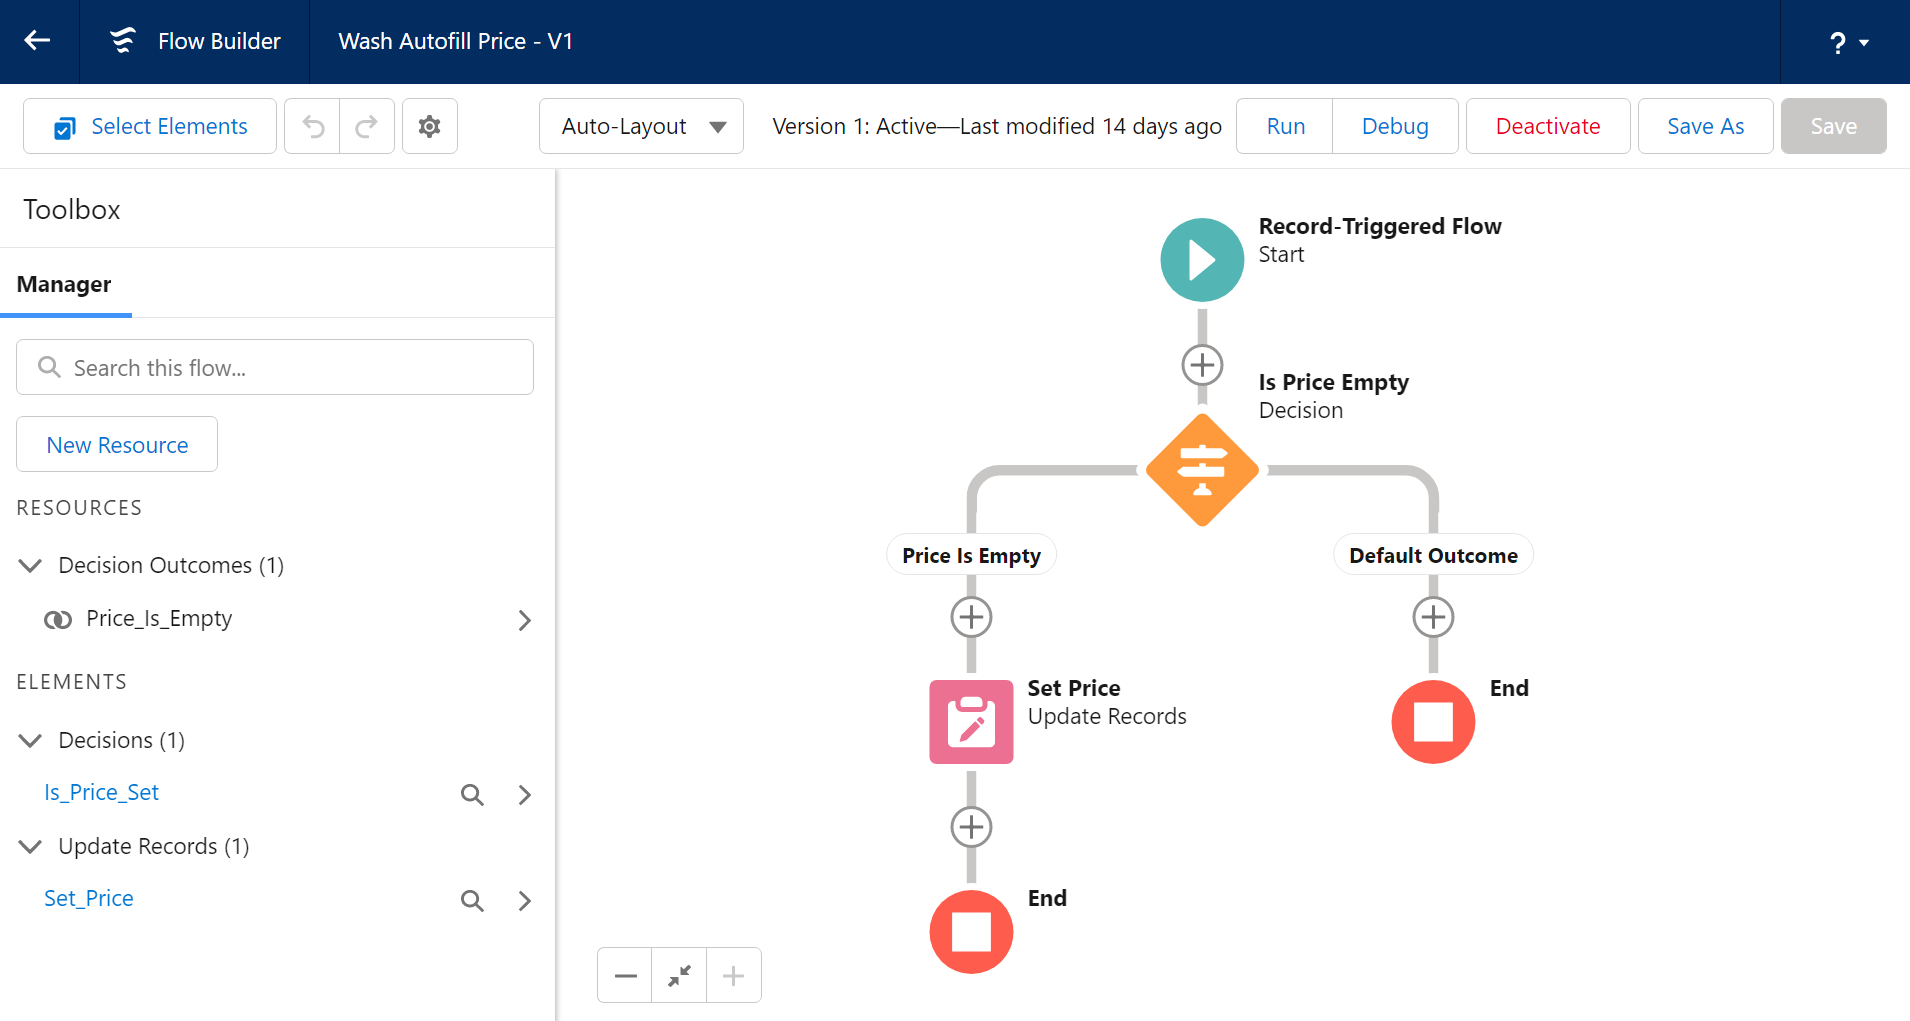
\includegraphics[width=\textwidth]{assets/7_implementace/automatizace/wash price autofill flow.png}
    \caption{Vyplnění ceny mytí ve vizuálním nástroji Flows.}
    \label{fig:wash_price_autofill_flow}
\end{figure}
\FloatBarrier
%%%%%%%%%%%%%%%%%%%%%%%%%%%%
\subsection{Vyplnění konce přezutí}
Pro zrychlení zadávání objednávek na přezutí byl automatizován koncový čas přezutí. Každé přezutí je nějakého typu, a každý typ má své trvání.

Příkladem může být přezutí celých kol, které může trvat 15 minut nebo složitější výměna pneumatik, která může trvat i 40 minut.

Přezutí nemusí mít zapsáno datum a čas konání. Ale v případě, že uživatel zapíše počáteční datum a čas, a nevyplní koncový datum a čas, do systému se propíše koncový čas podle trvání typu přezutí.

Této funkcionality bylo dosaženo pomocí starších \emph{Workflow Actions} s \emph{Workflow Rules}, které umožňují pracovat s formulemi.
Výpočet koncového času je vidět na obrázku \ref{fig:wheel_chage_autofill_date} a pravidla pro spuštění na obrázku \ref{fig:wheel_chage_autofill_date_rules}.
\begin{figure}[h!]
    \centering
    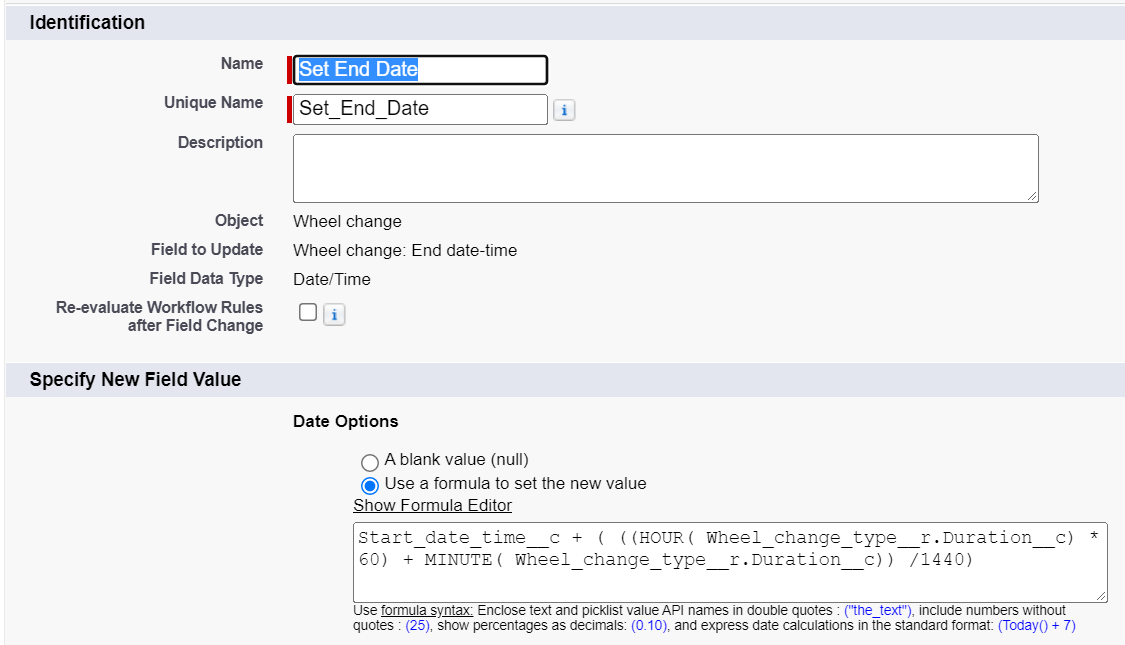
\includegraphics[width=\textwidth]{assets/7_implementace/automatizace/Wheel change end date Workflow Field Update.png}
    \caption{Aktualizace atributu konce přezutí podle formule}
    \label{fig:wheel_chage_autofill_date}
\end{figure}
\begin{figure}[h!]
    \centering
    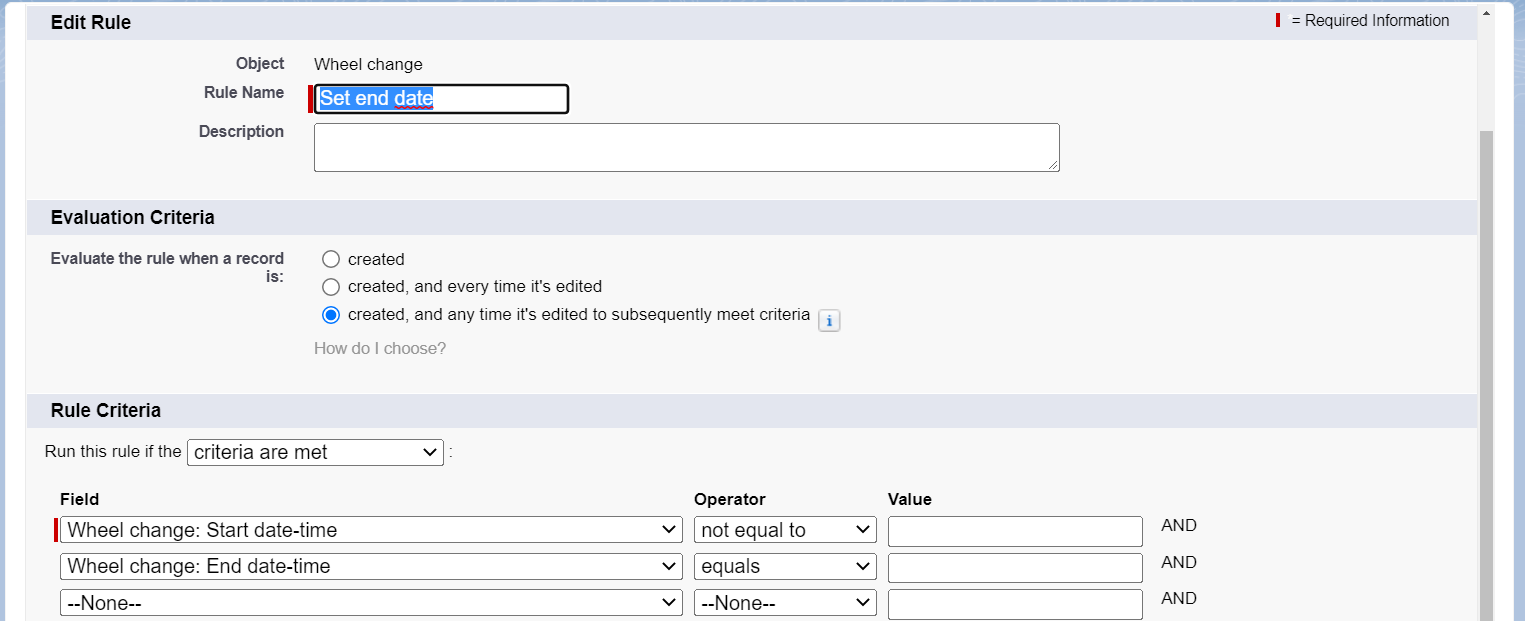
\includegraphics[width=\textwidth]{assets/7_implementace/automatizace/Workflow Rule.png}
    \caption{Pravidla pro spuštění Workflow Rule.}
    \label{fig:wheel_chage_autofill_date_rules}
\end{figure}
\FloatBarrier
%%%%%%%%%%%%%%%%%%%%%%%%%%%%
\subsection{Upozornění na objednané přezutí} \label{subsec:automation_wheel_change_notification}
Upozornění zákazníků na objednané přezutí je automatizováno pomocí vizuálního nástroje \emph{Flows} a je načasováno, aby se spustilo každý den v 10:00.

Upozornění je nastaveno tak, aby zkontrolovalo všechny objednávky na přezutí, a vybralo pouze ty, které se konají další den. 

V dalším kroku je provedena kontrola, zda má zákazník, kterého se přezutí týká, vyplněný e-mail. Poté systém odešle notifikační e-mail z adresy organizace. 

Po odeslání všech notifikačních e-mailů systém pošle notifikaci uživateli.

Konfigurace zprávy, kterou systém odesílá, se provádí úpravou proměnných, které obsahují text předmětu a text těla zprávy.
%%%%%%%%%%%%%%%%%%%%%%%%%%%%
\subsection{Upozornění na přezouvací sezónu} \label{subsec:automation_seasons}
Upozornění zákazníků na přezouvací sezónu je automatizováno pomocí vizuálního nástroje \emph{Flows} a atributů s formulí, které kontrolují datum. Tento proces se spouští každý den v 10:00.

Upozornění je nastaveno tak, aby vybralo všechny uživatele, kteří mají vyplněnou e-mailovou adresu a atribut zimní nebo atribut letní sezóny je nastaven na hodnotu \emph{True}. To zajistí odesílání pouze dvakrát v roce podle hodnoty těchto atributů.

Poté systém těmto zákazníkům odešle e-mail s upozorněním na začínající sezónu a notifikuje uživatele systému.

Konfigurace zprávy, kterou systém odesílá, se provádí úpravou proměnných, které obsahují text předmětu a text těla zprávy.
\begin{figure}[h!]
    \centering
    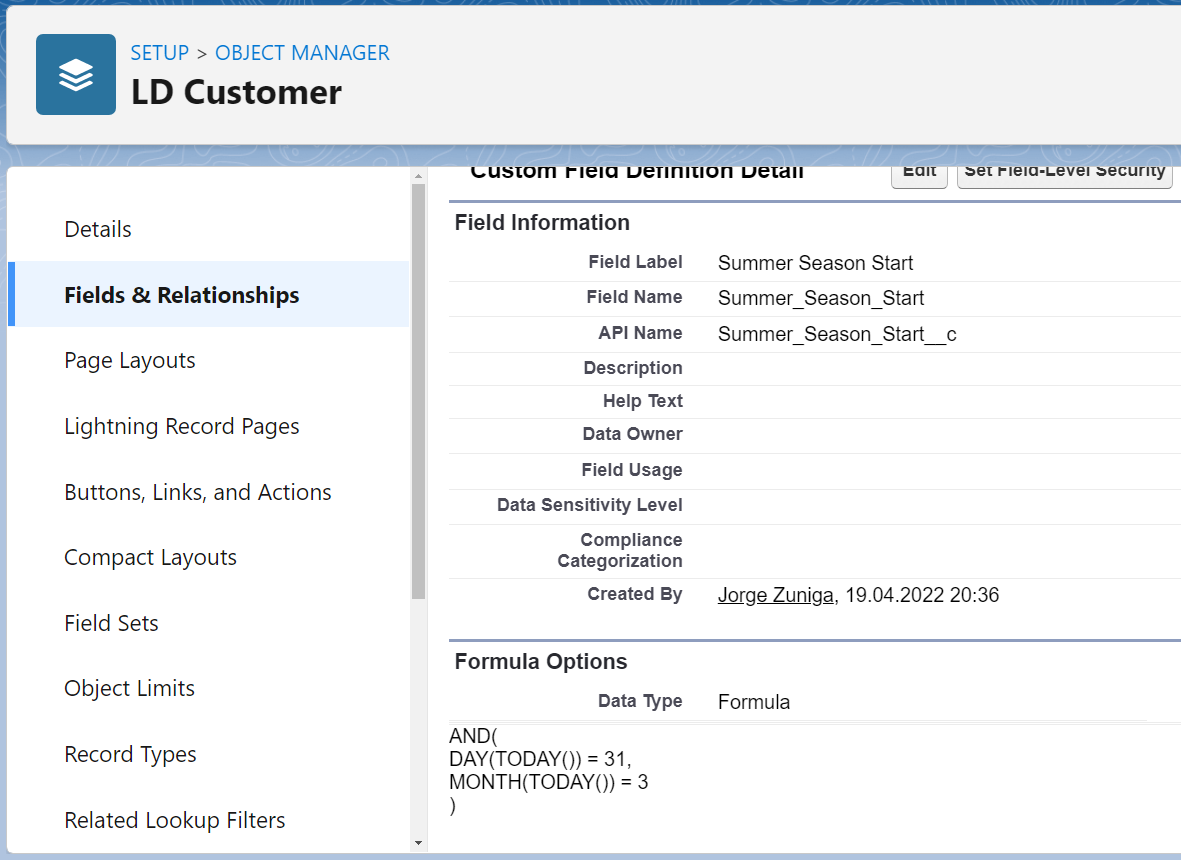
\includegraphics[width=\textwidth]{assets/7_implementace/automatizace/Summer season start.png}
    \caption{Atribut s formulí pro kontrolu začátku sezóny.}
    \label{fig:summer_season_start}
\end{figure}
\FloatBarrier
